\chapter{Gestión del proyecto}
\label{anx:gestion}


%%% Revisar las fechas y las horas

La realización de este proyecto comenzó a finales de septiembre de 2011 y se ha prolongado hasta agosto de 2012. A lo largo del mismo se han atravesado las fases de documentación, desarrollo, pruebas y redacción de la memoria. A continuación se muestra una tabla con las distintas fases y el coste en horas de cada una de ellas:

\begin{table}[!htbp]
\centering
   \begin{tabular}{|c|c|c|c|}
      \hline
      \textbf{Fase} & \textbf{Fecha de inicio} & \textbf{Fecha de finalización} & \textbf{Número de horas} \\ \hline
      Documentación & 29/09/2011 & 08/12/2011 & 148 \\ \hline
      Desarrollo & 13/12/2011 & XX/08/2012 & 380 \\ \hline
      Pruebas & 02/05/2012 & 02/07/2012 & 32 \\ \hline
      Memoria & 06/03/2012 & XX/08/2012 & 64 \\ \hline
      \hline
      Número total de horas & 29/09/2011 & XX/08/2012 & XX \\ \hline
   \end{tabular}
\caption{Número de horas invertidas.}
\label{table:horas}
\end{table}

Para ver el desarrollo del proyecto a lo largo de los meses se incluye a continuación un diagrama de Gantt:

\begin{figure} [!htbp]
  \centering
  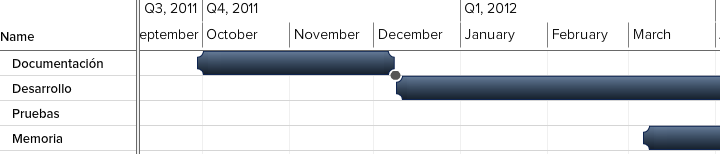
\includegraphics[width=13.5cm]{imagenes/gantt1.png}
  \caption{Diagrama de Gantt: septiembre a febrero.}
\label{figure:gantt1}
\end{figure}

\begin{figure} [!htbp]
  \centering
  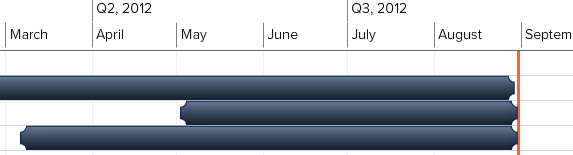
\includegraphics[width=13.5cm]{imagenes/gantt2.png}
  \caption{Diagrama de Gantt: marzo a agosto.}
\label{figure:gantt2}
\end{figure}

Como se puede observar, la fase del proyecto que más tiempo ha tomado ha sido la de desarrollo. En esta fase hubo tres cuestiones que tomaron bastante tiempo.

La primera de ellas fue la falta de documentación en AppScale. A la hora de averiguar cómo funcionaba Neptune (el lenguaje usado para enviar los trabajos MPI), ni la documentación que se podía encontrar en la página web, ni la documentación a la que se podía acceder una vez instalado eran suficientes. Después de enviar un correo electrónico preguntando por la información necesaria para poder trabajar con Neptune se creó la página web que ahora alberga la información relativa a los distintos trabajos que existen en Neptune.

La segunda de ellas fue un fallo en la parte de ejecución de los trabajos MPI. A la hora de copiar al nodo correspondiente el archivo que debía ejecutarse, no se tenían en cuenta los permisos de ejecución y, por lo tanto, se intentaba ejecutar un archivo sin los permisos necesarios. Encontrar y solucionar este bug consumió una buena parte de tiempo.

La tercera cuestión fue un fallo en el planificador de TORQUE. El planificador más básico que usa TORQUE, una cola FIFO, simplemente no funciona en la versión 4.0.2 y los trabajos nunca se llegaban a ejecutar. Aunque actualizar a la versión 4.0.3 solucionó el problema, no es un tipo de fallo que uno espera encontrar, y el hecho de ser una tecnología con la que nunca antes había trabajado no ayudó mucho en este aspecto.
